% ==================================================
% CHAPTER 6: RESULTS AND CONCLUSION
% ==================================================

\chapter{Results and Conclusion}
\label{ch:results}

\section{Results and Evaluation}

Table~\ref{tab:objectives} compares what was delivered with the objectives of
Section~1.2. Values marked as measured come from runs on 19--26~November 2026;
nothing in the table is an estimate.

\begin{table}[H]
\centering
\footnotesize
\begin{tabularx}{\textwidth}{>{\ttfamily}p{0.05\textwidth} >{\raggedright\arraybackslash}p{0.28\textwidth} L p{0.08\textwidth}}
\toprule
\textrm{\textbf{Obj.}} & \textbf{Objective} & \textbf{Delivered outcome} & \textbf{Status} \\
\midrule
O1 & Save pages; never store private pages & Manual and automatic capture; private pages refused twice (TC-04) & Met \\
O2 & Searchable by meaning and words & Cleaning, 150-word chunks, BGE vectors, BM25 + KNN in one core & Met \\
O3 & Right page first for most queries & Measured: Hit@1 0.71, Hit@10 0.93, MRR@10 0.786 on SciFact & Met \\
O4 & Private libraries; public HTTPS deployment & Isolation in the data layer (TC-16); live at \texttt{memorylane.site} & Met \\
O5 & Measure and improve retrieval & Seven metrics, latency, intervals; found and fixed a ranking defect & Met \\
O6 & Engineering practice & Specified and traced requirements; 11 ADRs; 566 tests in CI; documentation site & Met \\
\bottomrule
\end{tabularx}
\caption{Objectives and delivered outcomes}
\label{tab:objectives}
\end{table}

\subsection{Retrieval Evaluation}
\label{sec:evaluation}

\subsubsection{Benchmark}

Retrieval is evaluated on \textbf{SciFact} \cite{wadden2020scifact}, a
scientific-claim retrieval task from the BEIR benchmark
\cite{thakur2021beir}, adapted to MemoryLane's data model:

\begin{itemize}
  \item 1{,}000 SciFact abstracts saved as pages, each with a synthetic
  address of the form \path{https://scifact.org/doc/{id}}; 999 were indexed
  (one abstract fails cleaning and is not the answer to any claim);
  \item 100 claims as queries, with 115 claim--abstract relevance pairs.
\end{itemize}

The benchmark uses the production code end to end: abstracts are saved
through \texttt{ingest\_page} (cleaning, chunking, embedding, indexing) and
queries go through \texttt{hybrid\_search}, the function behind
\texttt{POST /search}. Everything runs in a separate Solr core under a
dedicated user id, so benchmark data never mixes with real libraries. The
final runs used a throwaway Solr 9.7 container on a laptop.

\subsubsection{Metrics}

The prototype reported three metrics. The final evaluation reports seven
quality metrics, two behaviour metrics, latency, and confidence intervals.
With $Q$ the claims, $\text{rel}_q$ the relevant abstracts of claim $q$, and
$r_q$ the rank of its first relevant result:

\begin{align*}
\text{Hit@}k &= \frac{1}{|Q|}\sum_{q} \mathbf{1}[r_q \leq k],
\qquad\qquad
\text{MRR@10} = \frac{1}{|Q|}\sum_{q} \frac{\mathbf{1}[r_q \le 10]}{r_q}, \\[2mm]
\text{Recall@10} &= \frac{1}{|Q|}\sum_{q} \frac{|\text{top}_{10}(q) \cap \text{rel}_q|}{|\text{rel}_q|}, \\[2mm]
\text{nDCG@10} &= \frac{1}{|Q|}\sum_{q}\frac{\sum_{i \le 10} \mathbf{1}[d_i \in \text{rel}_q]\,/\log_2(i+1)}{\sum_{i \le \min(10,|\text{rel}_q|)} 1/\log_2(i+1)},
\end{align*}

and MAP@10, the mean over claims of the precision at each relevant result in
the top ten \cite{manning2008ir,jarvelin2002ndcg}. The run also records the
empty rate (claims with no results, which the relevance floor could cause),
in-process latency at the median and 95th percentile, and bootstrap 95\% intervals for Hit@1 and MRR@10 (2{,}000 resamples) \cite{efron1993bootstrap}.
Every claim is searched once untimed first, so no configuration pays for
cold caches.

\paragraph{Configurations.} Five configurations were run, each by changing one setting for that run
only: \textbf{Hybrid} (the live search), \textbf{BM25 only},
\textbf{Vector only}, \textbf{Hybrid without the relevance floor}, and
\textbf{Hybrid with the old second-chunk bonus} (0.3).

\subsubsection{Results}

\begin{table}[H]
\centering
\small
\setlength{\tabcolsep}{2.4pt}
\begin{tabular}{lccccccc}
\toprule
\textbf{Configuration} & \textbf{Hit@1} & \textbf{Hit@3} & \textbf{Hit@10} & \textbf{MRR@10} & \textbf{R@10} & \textbf{nDCG@10} & \textbf{MAP@10} \\
\midrule
\textbf{Hybrid (live)} & 0.71 & 0.84 & 0.93 & 0.786 & 0.922 & 0.810 & 0.768 \\
BM25 only & 0.63 & 0.76 & 0.86 & 0.705 & 0.837 & 0.728 & 0.687 \\
Vector only & \textbf{0.75} & \textbf{0.86} & \textbf{0.94} & \textbf{0.812} & \textbf{0.932} & \textbf{0.837} & \textbf{0.803} \\
Hybrid, no floor & 0.71 & 0.84 & 0.93 & 0.785 & 0.922 & 0.810 & 0.768 \\
Hybrid, old bonus & 0.44 & 0.73 & 0.92 & 0.601 & 0.897 & 0.663 & 0.578 \\
\bottomrule
\end{tabular}
\caption{SciFact results for the final system (100 claims)}
\label{tab:results}
\end{table}

\begin{figure}[H]
\centering
\begin{tikzpicture}
\begin{axis}[
  ybar, bar width=9pt, width=\textwidth, height=6.2cm,
  ymin=0, ymax=1, ylabel={Score},
  symbolic x coords={Hit@1,Hit@3,Hit@10,MRR@10,nDCG@10,MAP@10},
  xtick=data, tick label style={font=\small},
  legend style={font=\scriptsize, at={(0.5,1.04)}, anchor=south, legend columns=4, draw=none,
                /tikz/every even column/.append style={column sep=4mm}},
  enlarge x limits=0.09, ymajorgrids, grid style={gray!25},
]
\addplot[fill=black!75] coordinates {(Hit@1,0.71) (Hit@3,0.84) (Hit@10,0.93) (MRR@10,0.786) (nDCG@10,0.810) (MAP@10,0.768)};
\addplot[fill=black!45] coordinates {(Hit@1,0.75) (Hit@3,0.86) (Hit@10,0.94) (MRR@10,0.812) (nDCG@10,0.837) (MAP@10,0.803)};
\addplot[fill=black!20] coordinates {(Hit@1,0.63) (Hit@3,0.76) (Hit@10,0.86) (MRR@10,0.705) (nDCG@10,0.728) (MAP@10,0.687)};
\addplot[fill=white, postaction={pattern=north east lines}] coordinates {(Hit@1,0.44) (Hit@3,0.73) (Hit@10,0.92) (MRR@10,0.601) (nDCG@10,0.663) (MAP@10,0.578)};
\legend{Hybrid (live), Vector only, BM25 only, Hybrid, old bonus}
\end{axis}
\end{tikzpicture}
\caption{Quality metrics by configuration}
\label{fig:results-bars}
\end{figure}

No claim received an empty result list in any configuration. Hybrid search
took \textbf{76\,ms} at the median and \textbf{93\,ms} at the 95th
percentile, in-process on a laptop (network and sign-in checks excluded).

\paragraph{Confidence.} With 100 claims, a few lucky or unlucky ones move an
average, so MRR@10 carries a bootstrap 95\% interval: 0.72--0.85 for hybrid
against 0.53--0.68 with the old bonus. The two do not overlap, so the
improvement is real; hybrid and vector-only (0.75--0.88) overlap almost
completely, so the gap between them may be chance.

\subsubsection{Finding: the Second-Chunk Bonus}
\label{sec:bonus}

Until this evaluation, a page scored its best chunk \emph{plus} 0.3 times its
second-best chunk, so that a page matching in two places would beat one
matching once. Under Reciprocal Rank Fusion, though, neighbouring ranks
score almost the same:

\[
\frac{1}{60+1} - \frac{1}{60+10} \approx 0.0021
\quad<\quad
0.3 \times \frac{1}{60+2} \approx 0.0048 .
\]

A single second match was therefore worth more than climbing nine places, and
\textbf{longer pages beat better matches}. When the old configuration put a
wrong abstract first, that abstract had 2.1 chunks on average; the right
answers had 1.3. A sweep of the bonus (Figure~\ref{fig:sweep}) showed every
non-zero value hurting, so the bonus was set to zero and pages are now
ranked by their best passage.

\begin{figure}[H]
\centering
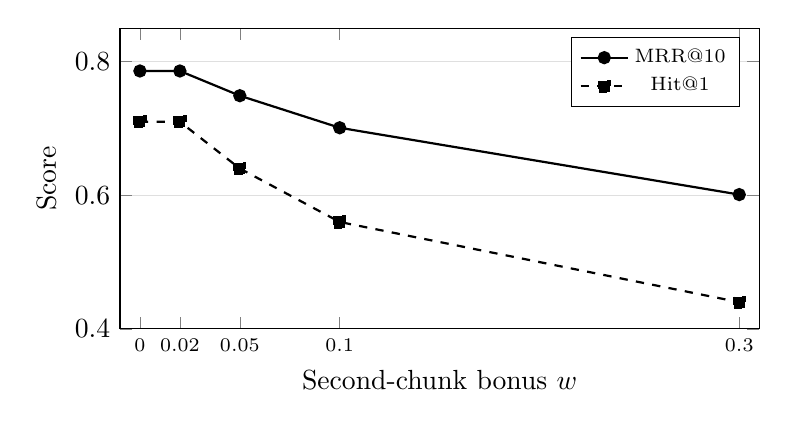
\begin{tikzpicture}
\begin{axis}[
  width=0.8\textwidth, height=5.4cm,
  xlabel={Second-chunk bonus $w$}, ylabel={Score},
  xmin=-0.01, xmax=0.31, ymin=0.4, ymax=0.85,
  xtick={0,0.02,0.05,0.1,0.3}, xticklabel style={font=\scriptsize, /pgf/number format/fixed},
  legend style={font=\scriptsize, at={(0.97,0.97)}, anchor=north east},
  ymajorgrids, grid style={gray!25}, mark size=2pt,
]
\addplot[thick, mark=*] coordinates {(0,0.786) (0.02,0.786) (0.05,0.749) (0.1,0.701) (0.3,0.601)};
\addplot[thick, dashed, mark=square*] coordinates {(0,0.71) (0.02,0.71) (0.05,0.64) (0.1,0.56) (0.3,0.44)};
\legend{MRR@10, Hit@1}
\end{axis}
\end{tikzpicture}
\caption{Effect of the second-chunk bonus on hybrid search}
\label{fig:sweep}
\end{figure}

\paragraph{Other findings.} Removing the relevance floor changed MRR@10 by
only 0.001: it drops weak vector-only matches, which on SciFact are rarely
right, and in real libraries keeps unrelated pages off short result lists.
Hybrid and vector-only are level because SciFact claims rarely share exact
words with their abstracts; hybrid is kept because everyday queries contain
names, error messages, product codes and sites that vector search can miss.

\paragraph{Comparison with the prototype.} Every configuration of the final
system beats its prototype counterpart on every metric. MRR@10 rose from
0.648 to 0.705 for BM25, from 0.780 to 0.812 for vector search, and from 0.754
(min-max fusion) to 0.786 (RRF) for hybrid search; Recall@10 and nDCG@10
moved the same way. The gains come from the stronger embedding model,
smaller overlapping chunks embedded with titles, rank fusion and
best-passage page scoring.

\subsubsection{Evaluation on a Personal Library}

SciFact measures scientific claims, not how people look for pages they have
read. A second evaluation runs on a real library with queries written by its
owner, each labelled \emph{navigational}, \emph{site}, \emph{topic} or
\emph{time}, and reports Recall@1/3/5/10 and MRR per category, with a
compare tool that lists every query whose rank changed. It was used to
measure site, time and URL understanding on a development library of 31
browsed pages among about 1{,}000 SciFact distractors:

\begin{table}[H]
\centering
\small
\begin{tabular}{lcccc}
\toprule
& \multicolumn{2}{c}{\textbf{Right page first}} & \multicolumn{2}{c}{\textbf{MRR}} \\
\cmidrule(lr){2-3}\cmidrule(lr){4-5}
\textbf{Query set} & before & after & before & after \\
\midrule
35 queries used while building & 0.86 & 0.94 & 0.900 & 0.971 \\
18 held-out queries & 0.72 & 0.94 & 0.787 & 0.944 \\
\bottomrule
\end{tabular}
\caption{Effect of site and time understanding on a personal library}
\label{tab:personal}
\end{table}

Most of the gain is in site queries (held-out MRR 0.75 $\rightarrow$ 1.00)
and time queries (0.38 $\rightarrow$ 1.00); topic-only queries are
unaffected, as intended. The sets are small, so the results indicate
direction rather than precise size.

\section{Challenges and Solutions}

\begin{table}[H]
\centering
\footnotesize
\begin{tabularx}{\textwidth}{>{\raggedright\arraybackslash}p{0.22\textwidth} L L L}
\toprule
\textbf{Challenge} & \textbf{Cause} & \textbf{Alternatives considered} & \textbf{Solution} \\
\midrule
Keeping keyword and vector search in step & Two stores (ChromaDB and a BM25 index) & Keep both; a hosted vector database & One Solr core for both (ADR 0001) \\
Combining scores on different scales & BM25 scores and cosines are not comparable & Min-max averaging; learned weights & Rank fusion with RRF (ADR 0002) \\
Weak results always shown & KNN always returns neighbours & Fixed result count; higher thresholds & Relevance floor and keyword coverage (ADR 0003) \\
Private pages captured automatically & Rules lived only in an outdated extension & A longer list of blocked sites & Content and reading rules, re-checked by the server (ADR 0011) \\
YouTube refused the server & YouTube blocks server transcript requests & A proxy; a paid API & Fetch captions in the user's browser (ADR 0006) \\
Two sign-ins, two libraries & Cognito gives Google and email different ids & One library per sign-in & Link by verified email (ADR 0005) \\
Search got worse after the rebuild & A page bonus outweighed RRF rank gaps & Smaller bonus values & Score pages by their best chunk (Section~\ref{sec:bonus}) \\
\bottomrule
\end{tabularx}
\caption{Challenges, alternatives and solutions}
\label{tab:challenges}
\end{table}

\section{Limitations and Scaling}

\paragraph{Limitations.} SciFact is a scientific benchmark and the
personal-library query sets are small, so neither fully represents everyday
browsing. Pages that render little text, videos without captions and content
behind logins are saved poorly or not at all. Page text is stored on the
server, and summaries send one page to an external model when asked, so users
must trust the operator. The extension targets Chromium browsers and is
installed unpacked.

\paragraph{Bottlenecks.} Embedding runs on the server's two CPU cores in one
process: it dominates the cost of saving a page (passages are embedded in
batches of 32), while a search embeds only the query (cached) and takes
about 76\,ms. Solr's 1\,GB heap and the 4\,GB of RAM bound the size of the
index on one machine.

\paragraph{Failure and recovery.} Every container restarts after a crash or
reboot, and health checks restart unhealthy services. If Gemini fails,
summaries are unavailable and everything else works; if email fails, reports
wait in SQLite and are retried; if Cognito is unreachable, known sign-ins keep
working. Losing the server would lose data newer than the last EBS snapshot,
the main operational risk of the single-server design (ADR 0004).

\paragraph{Scaling up and down.} The backend is stateless apart from its
SQLite files, so more users can be served by moving SQLite to a managed
database and running several backend replicas behind Caddy, with Solr in
SolrCloud mode for a larger index. To scale down, the reranker is already off
and summaries are optional; the whole system fits on one small instance. The
running cost is one \texttt{c7i-flex.large} instance plus free tiers of
Cognito, SES and Gemini; more users would add mainly CPU for embedding and
memory for Solr.

\section{Individual Contributions}

\begin{table}[H]
\centering
\footnotesize
\begin{tabularx}{\textwidth}{>{\raggedright\arraybackslash}p{0.17\textwidth} L}
\toprule
\textbf{Member} & \textbf{Specific work} \\
\midrule
Rabeeh Ahmad (\texttt{1024030716}) & Project proposal and meeting overview; move to Apache Solr and hybrid search; automatic capture and the page filter; URL normalisation; the evaluation pipeline and the SciFact evaluations; the mid-semester and final reports; the October rebuild (retrieval, ingestion and schema v2, Cognito sign-in and isolation, new web app and extension, Docker Compose and Caddy deployment); site and time understanding; account linking; problem reports; the bug audit and fixes; the ranking fix; the documentation site. \\
Ishan Singhania (\texttt{1024030719}) & The first working prototype (TamperMonkey script and backend code) and its forum announcement; YouTube transcript support; voice search and its later fix; the Vercel deployment of the first web app; the Version~2 forum update; the product demo video. \\
Shared & Project idea and design discussions with the supervisor; weekly forum updates; testing the live system. \\
\bottomrule
\end{tabularx}
\caption{Individual contributions}
\label{tab:contributions}
\end{table}

\section{Conclusion}

MemoryLane turns the pages a person reads into a memory they can search by
describing what they remember. Over the semester it grew from a single-user
prototype into a deployed, multi-user product: a Chrome extension that saves
pages and videos and captures automatically only what was read and looks like
content; a hybrid search that fuses BM25 and vector retrieval by rank,
understands sites and times, filters weak matches and shows readable snippets;
and a web app with a library, undoable deletes, summaries and voice search,
behind Cognito sign-in with isolation enforced in the data layer. On SciFact
the live search puts the right abstract first for 71\% of claims and in the
top ten for 93\%, ahead of the prototype on every metric, in about 76\,ms.

\paragraph{Lessons learned.} Measuring matters as much as building: the
largest single improvement of the semester came from evaluating the system
honestly and fixing what the numbers revealed. Security is easiest when it is
built into one layer (the Solr client) rather than repeated in every endpoint.
And features should earn their place: removing the library map and export made
the product simpler without losing anything users relied on.

\section{Future Work}
\label{sec:future}

\begin{enumerate}
  \item \textbf{Broader evaluation}: more BEIR datasets and a larger personal
  query set, run automatically after every retrieval change.
  \item \textbf{End-to-end and accessibility testing}: browser tests of the
  main flows, an accessibility audit, and a load test at the page limit.
  \item \textbf{Learned reranking}: enable the cross-encoder where memory
  allows, and measure it.
  \item \textbf{Summary fallback}: a second, cheaper model or an extractive
  summary when Gemini is unavailable.
  \item \textbf{Import}: bring in existing bookmarks and browser history.
  \item \textbf{Account features}: password change and signing out of every
  device.
  \item \textbf{Local-first mode}: on-device embedding and storage for users
  who do not want page text on a server.
  \item \textbf{Store distribution}: publish the extension in the Chrome Web
  Store, and port it to Firefox.
\end{enumerate}
